\documentclass[]{article}
\usepackage{lmodern}
\usepackage{amssymb,amsmath}
\usepackage{ifxetex,ifluatex}
\usepackage{fixltx2e} % provides \textsubscript
\ifnum 0\ifxetex 1\fi\ifluatex 1\fi=0 % if pdftex
  \usepackage[T1]{fontenc}
  \usepackage[utf8]{inputenc}
\else % if luatex or xelatex
  \ifxetex
    \usepackage{mathspec}
  \else
    \usepackage{fontspec}
  \fi
  \defaultfontfeatures{Ligatures=TeX,Scale=MatchLowercase}
\fi
% use upquote if available, for straight quotes in verbatim environments
\IfFileExists{upquote.sty}{\usepackage{upquote}}{}
% use microtype if available
\IfFileExists{microtype.sty}{%
\usepackage{microtype}
\UseMicrotypeSet[protrusion]{basicmath} % disable protrusion for tt fonts
}{}
\usepackage[margin=1in]{geometry}
\usepackage{hyperref}
\hypersetup{unicode=true,
            pdftitle={transmission\_metrics},
            pdfauthor={Paul Taconet},
            pdfborder={0 0 0},
            breaklinks=true}
\urlstyle{same}  % don't use monospace font for urls
\usepackage{graphicx,grffile}
\makeatletter
\def\maxwidth{\ifdim\Gin@nat@width>\linewidth\linewidth\else\Gin@nat@width\fi}
\def\maxheight{\ifdim\Gin@nat@height>\textheight\textheight\else\Gin@nat@height\fi}
\makeatother
% Scale images if necessary, so that they will not overflow the page
% margins by default, and it is still possible to overwrite the defaults
% using explicit options in \includegraphics[width, height, ...]{}
\setkeys{Gin}{width=\maxwidth,height=\maxheight,keepaspectratio}
\IfFileExists{parskip.sty}{%
\usepackage{parskip}
}{% else
\setlength{\parindent}{0pt}
\setlength{\parskip}{6pt plus 2pt minus 1pt}
}
\setlength{\emergencystretch}{3em}  % prevent overfull lines
\providecommand{\tightlist}{%
  \setlength{\itemsep}{0pt}\setlength{\parskip}{0pt}}
\setcounter{secnumdepth}{0}
% Redefines (sub)paragraphs to behave more like sections
\ifx\paragraph\undefined\else
\let\oldparagraph\paragraph
\renewcommand{\paragraph}[1]{\oldparagraph{#1}\mbox{}}
\fi
\ifx\subparagraph\undefined\else
\let\oldsubparagraph\subparagraph
\renewcommand{\subparagraph}[1]{\oldsubparagraph{#1}\mbox{}}
\fi

%%% Use protect on footnotes to avoid problems with footnotes in titles
\let\rmarkdownfootnote\footnote%
\def\footnote{\protect\rmarkdownfootnote}

%%% Change title format to be more compact
\usepackage{titling}

% Create subtitle command for use in maketitle
\providecommand{\subtitle}[1]{
  \posttitle{
    \begin{center}\large#1\end{center}
    }
}

\setlength{\droptitle}{-2em}

  \title{transmission\_metrics}
    \pretitle{\vspace{\droptitle}\centering\huge}
  \posttitle{\par}
    \author{Paul Taconet}
    \preauthor{\centering\large\emph}
  \postauthor{\par}
      \predate{\centering\large\emph}
  \postdate{\par}
    \date{24/03/2020}

\usepackage{booktabs}
\usepackage{longtable}
\usepackage{array}
\usepackage{multirow}
\usepackage{wrapfig}
\usepackage{float}
\usepackage{colortbl}
\usepackage{pdflscape}
\usepackage{tabu}
\usepackage{threeparttable}
\usepackage{threeparttablex}
\usepackage[normalem]{ulem}
\usepackage{makecell}
\usepackage{xcolor}

\begin{document}
\maketitle

\hypertarget{introduction}{%
\section{Introduction}\label{introduction}}

La lutte contre la transmission du paludisme repose aujourd'hui
essentiellement sur l'utilisation de moustiquaires imprégnées
d'insecticides à longue durée d'action (MILDAs). La réduction de
l'incidence du paludisme due à l'utilisation des MILDAs a été largement
documentée et prouvée. Cependant, on observe que la transmission
persiste dans les sites où cette méthode de lutte anti-vectorielle (LAV)
est mise en œuvre. On définit alors par transmission résiduelle du
paludisme toute forme de transmission de la maladie qui persiste après
la mise en place d'outils de LAV. Bien que les conditions favorisant la
transmission résiduelle sont encore peu documentées, il est reconnu que
cette dernière est la conséquence de changements de composition
spécifique des populations de vecteurs, ainsi que de l'émergence de
mécanismes de résistances - physiologiques ou comportementaux - à la LAV
au sein de ces populations. Les phénotypes résistants dans les
population de vecteurs peuvent alors transmettre le parasite responsable
du paludisme aux populations humaines, bien que ces dernières utilisent
les MILDAs. Par ailleurs, les conditions d'utilisation effective des
MILDAs rendent les populations plus ou moins vulnérables aux piqûres et
influent ainsi sur la transmission résiduelle du paludisme.

La thèse consiste à améliorer la compréhension globale des phénomènes
entrant en jeu dans le risque de transmission résiduelle du paludisme.
Ce risque dépend en partie des probabilités de présence, densité
agressive et prévalence de phénotypes résistants des vecteurs, ainsi que
des conditions d'utilisation effective des MILDAs par les populations
humaines. Ces variables dépendent elles-mêmes en grande partie de
l'environnement dans lesquels les populations, humaines et vectorielles,
évoluent (paysage, conditions climatiques, outils de LAV, etc.). Les
travaux s'attacheront donc à décrire, quantifier et prévoir les
différentes composantes du risque de transmission résiduelle
sus-mentionnées en fonction des composantes environnementales, à l'aide
de méthodes de modélisation mathématique. Les objectifs sont i)
d'améliorer les connaissances fondamentales sur les déterminants de la
transmission résiduelle et ii) de proposer une méthode de prédiction du
risque de transmission à de fines échelles spatiales et temporelles en
utilisant des données terrain ponctuelles et des données satellitaires.

Les données de terrain utilisées pour les travaux sont issues de
campagnes épidémiologiques, entomologiques et sociologiques effectuées
dans des villages au Sud du Burkina Faso et au Nord de la Côte d'Ivoire
dans le cadre d'un projet de recherche porté par l'IRD (projet REACT).
Ces données sont utilisées pour créer les séries statistiques à
expliquer et prévoir. Le projet REACT s'est attaché à étudier et mesurer
le bénéfice à utiliser 4 nouvelles stratégies de LAV en complément des
MILDAs : Information éducation et communication, les pulvérisations
intra-domiciliaires, l'utilisation d'ivermectine et la lutte
anti-larvaire.

Les variables explicatives / prédictives sont principalement issues de
produits satellitaires d'observation de la Terre.

\hypertarget{presentation-des-zones-detudes-du-projet-react}{%
\section{Présentation des zones d'études du projet
REACT}\label{presentation-des-zones-detudes-du-projet-react}}

La carte suivante présente la localisation des villages de l'étude dans
les deux zones (BF = Burkina Faso ; CI = Côte d'Ivoire). Les villages
sont coloriés en fonction de la stratégie complémentaire de LAV
implémentée dans chaque village (à noter que la méthodologie utilisée
est un Essai randomisé contrôlé, ainsi, certains villages n'ont pas reçu
de statégie de lutte complémentaire : il s'agit des villages
``Contrôle'')

La figure ci-dessous présente le calendrier simplifié du projet :

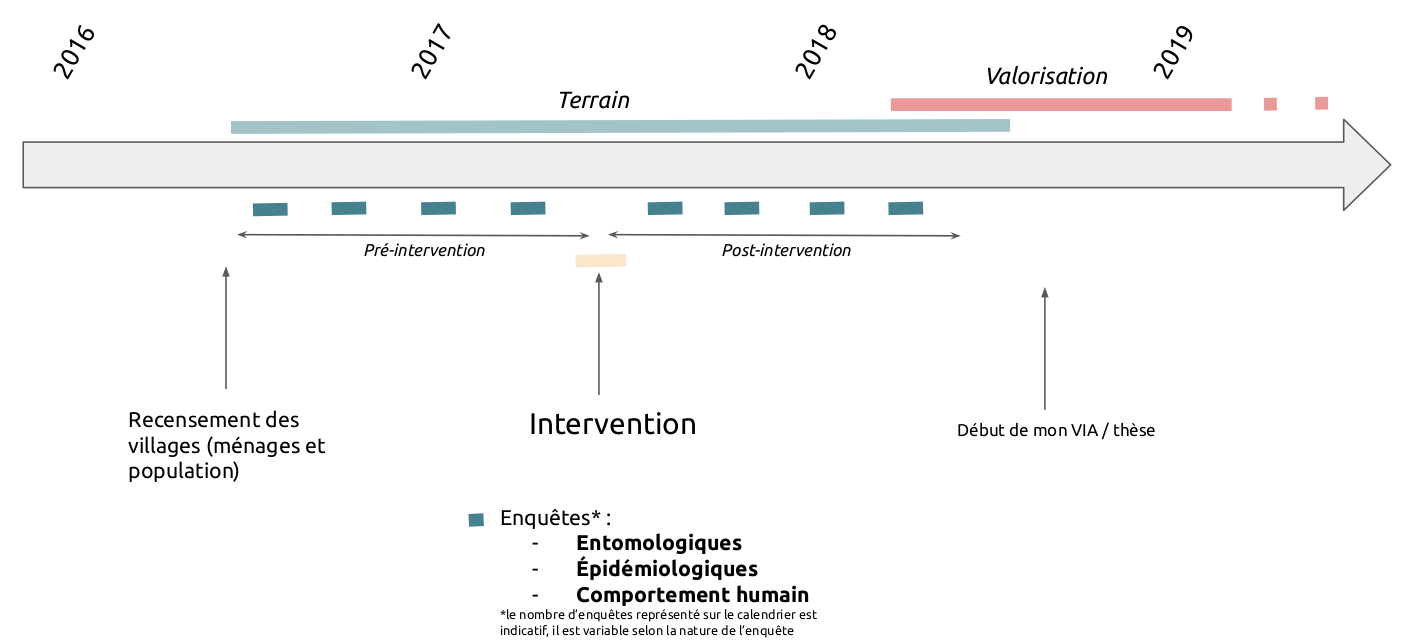
\includegraphics{references/figures/calendar_react.png}

\hypertarget{variables-a-expliquer-prevoir}{%
\section{Variables à expliquer /
prévoir}\label{variables-a-expliquer-prevoir}}

Les variables que l'on va chercher à expliquer et prévoir sont données
dans le tableau ci - dessous. Il s'agit de variables entomologiques

Following indicators are provided for each study area :

\begin{table}[H]
\centering
\begin{tabular}{l|l|l|l|l}
\hline
code & short\_name & long\_name & ...4 & method\\
\hline
pres\_an & NA & NA & NA & random forest\\
\hline
ma\_an & Human biting rate (all Anopheles species) & Number of bites by Anopheles mosquitoes (bites / person / night) & NA & random forest\\
\hline
pres\_funestus\_ss & NA & NA & NA & NA\\
\hline
ma\_funestus\_ss & NA & NA & NA & NA\\
\hline
pres\_gambiae\_ss & NA & NA & NA & NA\\
\hline
ma\_gambiae\_ss & NA & NA & NA & NA\\
\hline
pres\_coluzzi & NA & NA & NA & NA\\
\hline
ma\_coluzzi & NA & NA & NA & NA\\
\hline
eir\_an & Entomological inoculation rate (all Anopheles species) & NA & NA & NA\\
\hline
NA & NA & Number of infectious bites by Anopheles mosquitoes (bites / person / night) & NA & NA\\
\hline
eir\_sp & Entomological inoculation rate (by major Anopheles species) & Number of infectious bites by Anopheles mosquitoes (bites / person / night) & NA & NA\\
\hline
sr\_an & Sporozoite rate (all Anopheles species) & Proportion of Anopheles with plasmodium falciparum sporozoites in their salivary glands & NA & NA\\
\hline
sr\_sp & Sporozoite rate (by major Anopheles species) & Proportion of Anopheles with plasmodium falciparum sporozoites in their salivary glands & NA & NA\\
\hline
er\_an & Exophagy rate (all Anopheles species) & Proportion of the Anopheles that bite outdoor & NA & NA\\
\hline
er\_sp & Exophagy rate (by major Anopheles species) & Proportion of the Anopheles that bite outdoor & NA & NA\\
\hline
spr\_tot & Slide positivity rate (children < 20 years old) & Proportion of those examined who test positive for parasitaemia & NA & NA\\
\hline
spr\_inf\_5 & Slide positivity rate (children < 5 years old) & Proportion of those examined who test positive for parasitaemia & NA & NA\\
\hline
spr\_5\_10 & Slide positivity rate (children > 5 y.o. and < 10 y.o.) & Proportion of those examined who test positive for parasitaemia & NA & NA\\
\hline
spr\_sup\_10 & Slide positivity rate (children > 10 years old) & Proportion of those examined who test positive for parasitaemia & NA & NA\\
\hline
NA & NA & NA & NA & NA\\
\hline
er\_funestus\_ss & Exophagy rate (an. funestus ss.) & Proportion of bites occuring outside (an. funestus ss.) & entomological & FALSE\\
\hline
er\_gambiae\_ss & Exophagy rate (an. gambiae ss.) & Proportion of bites occuring outside (an. gambiae ss.) & entomological & FALSE\\
\hline
er\_coluzzi & Exophagy rate (an. coluzzi) & Proportion of bites occuring outside (an. coluzzi ss.) & entomological & FALSE\\
\hline
bre\_an & Behavorial resistance (all anopheles) & Proportion of early and late biting & entomological & TRUE\\
\hline
bre\_funestus\_ss & NA & NA & NA & NA\\
\hline
bre\_gambiae\_ss & NA & NA & NA & NA\\
\hline
bre\_coluzzi & NA & NA & NA & NA\\
\hline
\end{tabular}
\end{table}

\hypertarget{pres_an}{%
\subsubsection{pres\_an}\label{pres_an}}

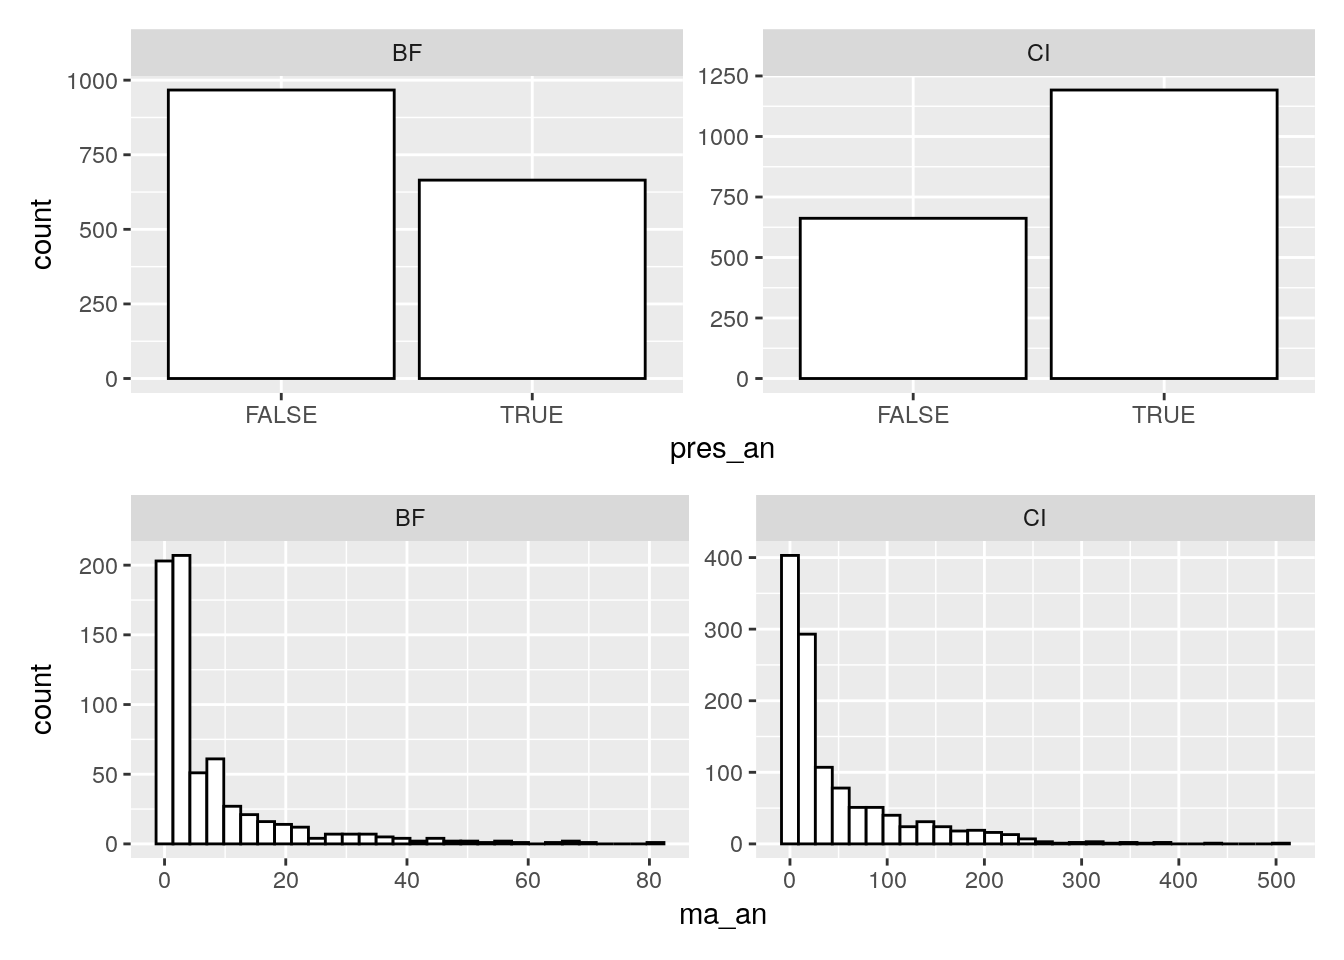
\includegraphics{transmission_metrics2_files/figure-latex/pres_an-1.pdf}

\hypertarget{ma_an}{%
\subsubsection{ma\_an}\label{ma_an}}

\includegraphics{transmission_metrics2_files/figure-latex/ma_an-1.pdf}
\includegraphics{transmission_metrics2_files/figure-latex/ma_an-2.pdf}

\hypertarget{pres_funestus_ss-pres_gambiae_ss-pres_coluzzi}{%
\subsubsection{pres\_funestus\_ss, pres\_gambiae\_ss,
pres\_coluzzi}\label{pres_funestus_ss-pres_gambiae_ss-pres_coluzzi}}

\includegraphics{transmission_metrics2_files/figure-latex/pres_sp-1.pdf}

\hypertarget{ma_funestus_ss-ma_gambiae_ss-ma_coluzzi}{%
\subsubsection{ma\_funestus\_ss, ma\_gambiae\_ss,
ma\_coluzzi}\label{ma_funestus_ss-ma_gambiae_ss-ma_coluzzi}}

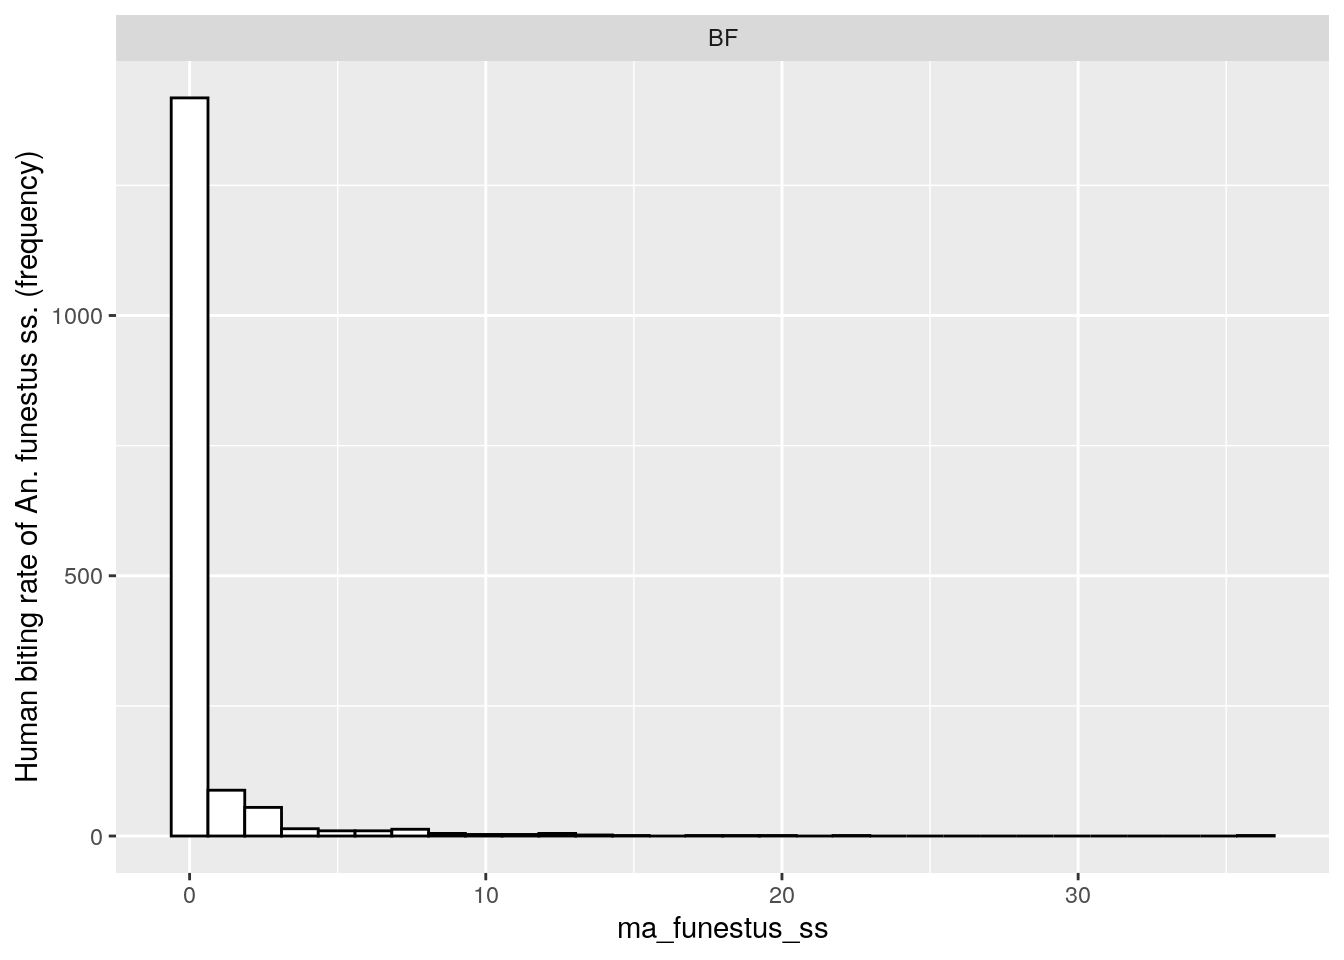
\includegraphics{transmission_metrics2_files/figure-latex/ma_sp-1.pdf}
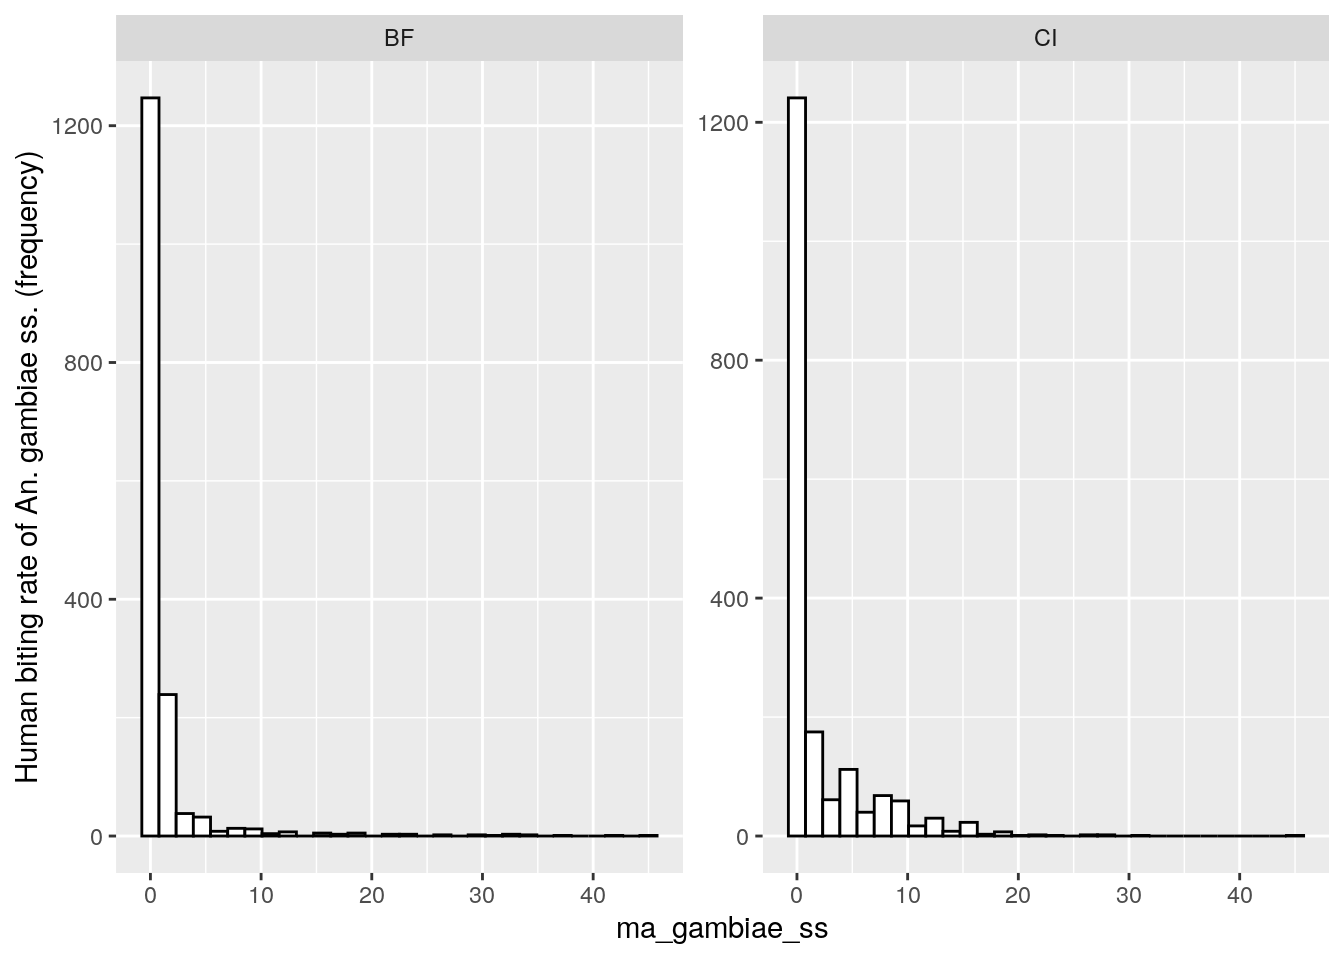
\includegraphics{transmission_metrics2_files/figure-latex/ma_sp-2.pdf}
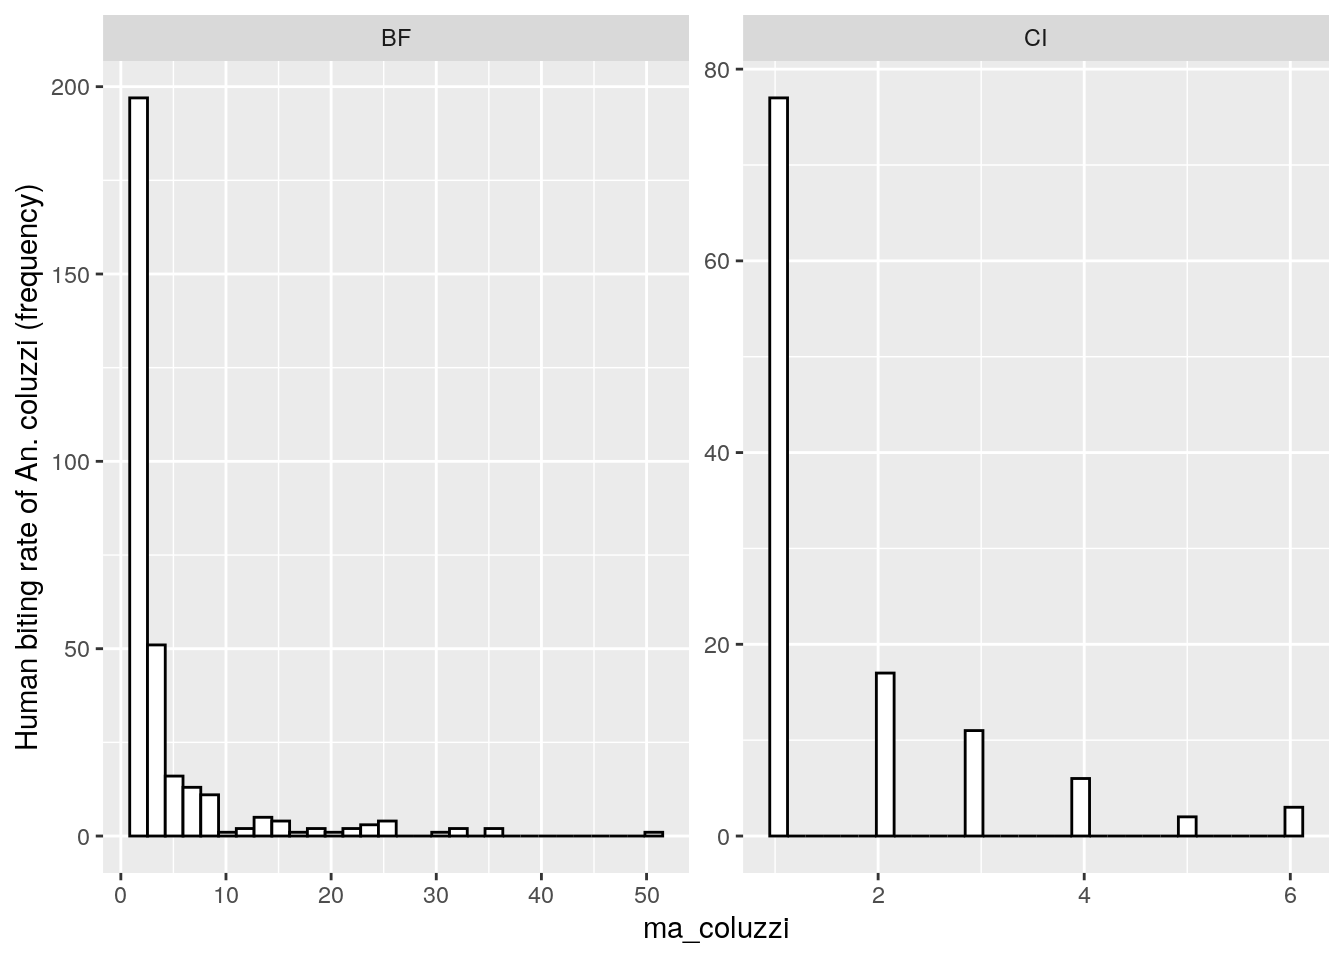
\includegraphics{transmission_metrics2_files/figure-latex/ma_sp-3.pdf}

\hypertarget{er_an}{%
\subsubsection{er\_an}\label{er_an}}

\hypertarget{er_funestus_ss-er_gambiae_ss-er_coluzzi}{%
\subsubsection{er\_funestus\_ss, er\_gambiae\_ss,
er\_coluzzi}\label{er_funestus_ss-er_gambiae_ss-er_coluzzi}}


\end{document}
